\appendix

%%%% Almost all weight are the same -- commenting this out

% \begin{table}[htbp]
%   \centering
%   \caption{%
%     Quality-factor metric weights $\lambda_i$ assigned to each dataset.
%     The weights enter the objective as
%     $L = \lambda_1 S_{\mathrm{BG}}
%     + \lambda_2 f_{\mathrm{neg,con}}
%     + \lambda_3 f_{\mathrm{neg,syn}}
%     + \lambda_4 \mathrm{NMSE}_{\mathrm{syn}}
%     + \lambda_5 (1 - f_{B})$.
%     The same $\lambda_i$ are used for all background removal methods.
%   }
%   \label{tab:weights_datasets}
%   \begin{tabular}{@{}l r r r r r@{}}
%     \toprule
%     {Dataset} &
%     {$\lambda_1$} &
%     {$\lambda_2$} &
%     {$\lambda_3$} &
%     {$\lambda_4$} &
%     {$\lambda_5$} \\
%     &
%     {($S_{\mathrm{BG}}$)} &
%     {($f_{\mathrm{neg,con}}$)} &
%     {($f_{\mathrm{neg,syn}}$)} &
%     {($\mathrm{NMSE}_{\mathrm{syn}}$)} &
%     {($1 - f_{B}$)} \\
%     \midrule
%     \texttt{2022\_1028} & 0.10 & 0.05 & 0.05 & 0.01 & 0.80 \\
%     \texttt{2024\_0508}                 & 0.10 & 0.05 & 0.05 & 0.01 & 0.80 \\
%     \texttt{2024\_1213\_air}             & 0.10 & 0.05 & 0.05 & 0.01 & 0.80 \\
%     \texttt{2024\_1213\_buffer}          & 0.10 & 0.05 & 0.05 & 0.01 & 0.80 \\
%     \texttt{2026\_0409\_air}                  & 0.10 & 0.05 & 0.05 & 0.01 & 0.80 \\
%     \texttt{2026\_0409\_sol}                  & 0.10 & 0.05 & 0.05 & 0.01 & 0.80 \\
%     \texttt{P2\_F6\_639}                      & 0.10 & 0.05 & 0.05 & 0.01 & 0.80 \\
%     \texttt{P3\_F4\_675}                      & 0.10 & 0.05 & 0.05 & 0.01 & 0.80 \\
%     \texttt{MPLL}              & 0.10 & 0.05 & 0.05 & 0.01 & 0.80 \\
%     % \addlinespace
%     \texttt{2025\_0227}                    & 0.10 & 0.05 & 0.05 & 0.001 & 0.80 \\
%     \texttt{2025\_0402}                 & 0.10 & 0.05 & 0.05 & 0.001 & 0.80 \\
%     \bottomrule
%   \end{tabular}
% \end{table}



Sensitivity to the synthetic signal parameters was also evaluated. Table~\ref{tab:synthetic_variations} summarizes results obtained under different synthetic feature configurations. The relatively small changes in aggregate loss across these conditions indicate that the evaluation framework is not overly sensitive to the precise choice of synthetic signal parameters.



\begin{table}[h]
\centering
\small
\begin{tabular}{lcccccccr}
\hline
Samp. Freq. & ($\sigma_x$, $\sigma_y$) & Loss & MSE$_{\mathbf{syn}}$ & \%Neg$_{\mathbf{con}}$ & \%Neg$_{\mathbf{syn}}$ & $1-\%\mathbf{B}'$ & $\mathbf{S}_{\mathbf{BG}}$ \\
\hline
dense & (5, 10) & $0.52 \pm 0.13$ & $5.10 \pm 4.57$ & $0.90 \pm 0.65$ & $1.09 \pm 0.39$ & $0.24 \pm 0.12$ & $1.89 \pm 0.33$ \\
medium & (5, 5) & $0.51 \pm 0.13$ & $4.17 \pm 4.21$ & $0.89 \pm 0.66$ & $1.07 \pm 0.41$ & $0.26 \pm 0.14$ & $1.82 \pm 0.26$ \\
medium & (3, 10) & $0.53 \pm 0.16$ & $5.36 \pm 5.22$ & $0.90 \pm 0.67$ & $1.09 \pm 0.35$ & $0.27 \pm 0.17$ & $1.84 \pm 0.19$ \\
medium & (7, 10) & $0.51 \pm 0.16$ & $3.70 \pm 4.47$ & $0.91 \pm 0.67$ & $1.01 \pm 0.40$ & $0.26 \pm 0.17$ & $1.87 \pm 0.20$ \\
medium & (5, 10) & $0.51 \pm 0.12$ & $3.61 \pm 3.52$ & $0.91 \pm 0.67$ & $1.05 \pm 0.40$ & $0.25 \pm 0.15$ & $1.85 \pm 0.20$ \\
medium & (5, 20) & $0.50 \pm 0.13$ & $3.33 \pm 3.41$ & $0.91 \pm 0.67$ & $1.05 \pm 0.40$ & $0.25 \pm 0.15$ & $1.86 \pm 0.20$ \\
sparse & (5, 10) & $0.51 \pm 0.12$ & $3.61 \pm 3.52$ & $0.91 \pm 0.67$ & $1.05 \pm 0.40$ & $0.25 \pm 0.15$ & $1.85 \pm 0.20$ \\
\hline
\end{tabular}
\caption{Sensitivity of the evaluation framework to variations in synthetic signal parameters. Values are reported as mean $\pm$ standard deviation across datasets. The purpose of this table is to demonstrate robustness of the aggregate loss to reasonable changes in synthetic feature configuration.}
\label{tab:synthetic_variations}
\end{table}



% \begin{figure}[htbp]
% \centering
% 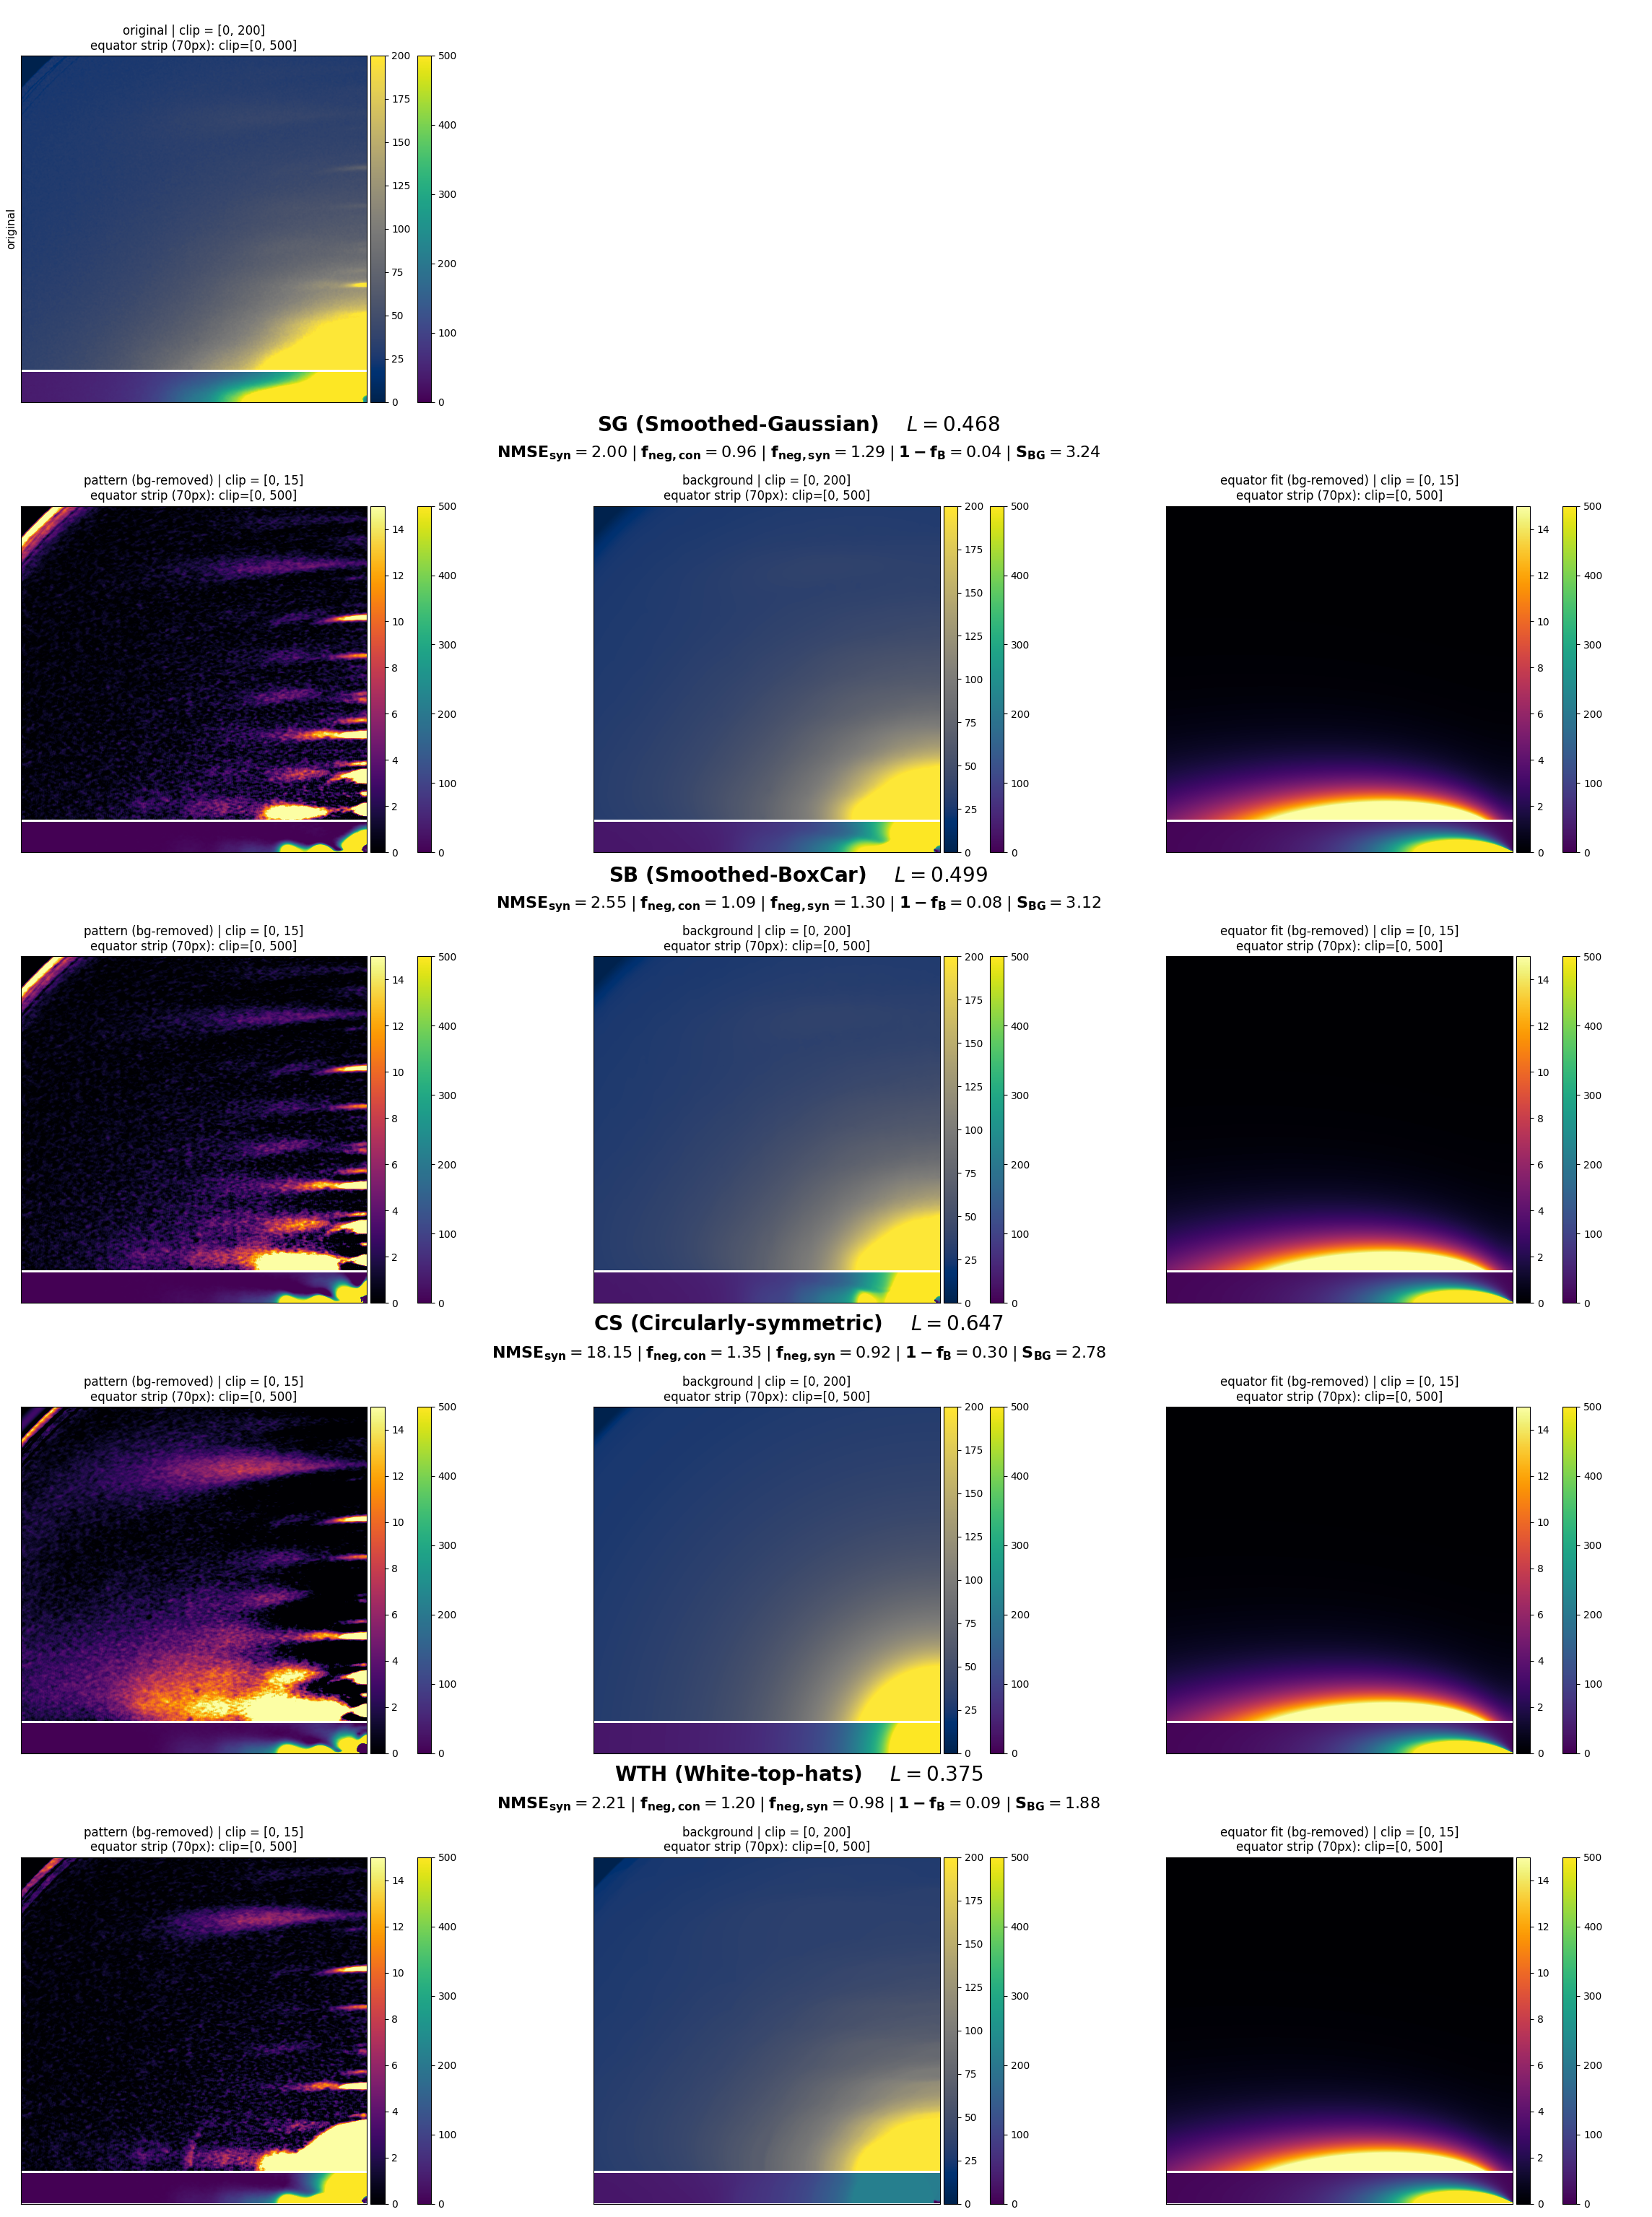
\includegraphics[height=0.9\textheight]{figs/example_eq_Jani_3_1.png}
% \caption{Visual comparison of background subtraction outcomes for image from dataset 2025\_0402 after equatorial streak fitting and general background removal. Left to right: background-subtracted pattern, background, fitted equatorial streak. The original image is shown at the top. Two scales are used for visualization due to high intensity differences between the background, the equatorial streak and the rest of the pattern.}
% \label{fig:visual_eq_1}
% \end{figure}


% \begin{figure}[htbp]
% \centering
% 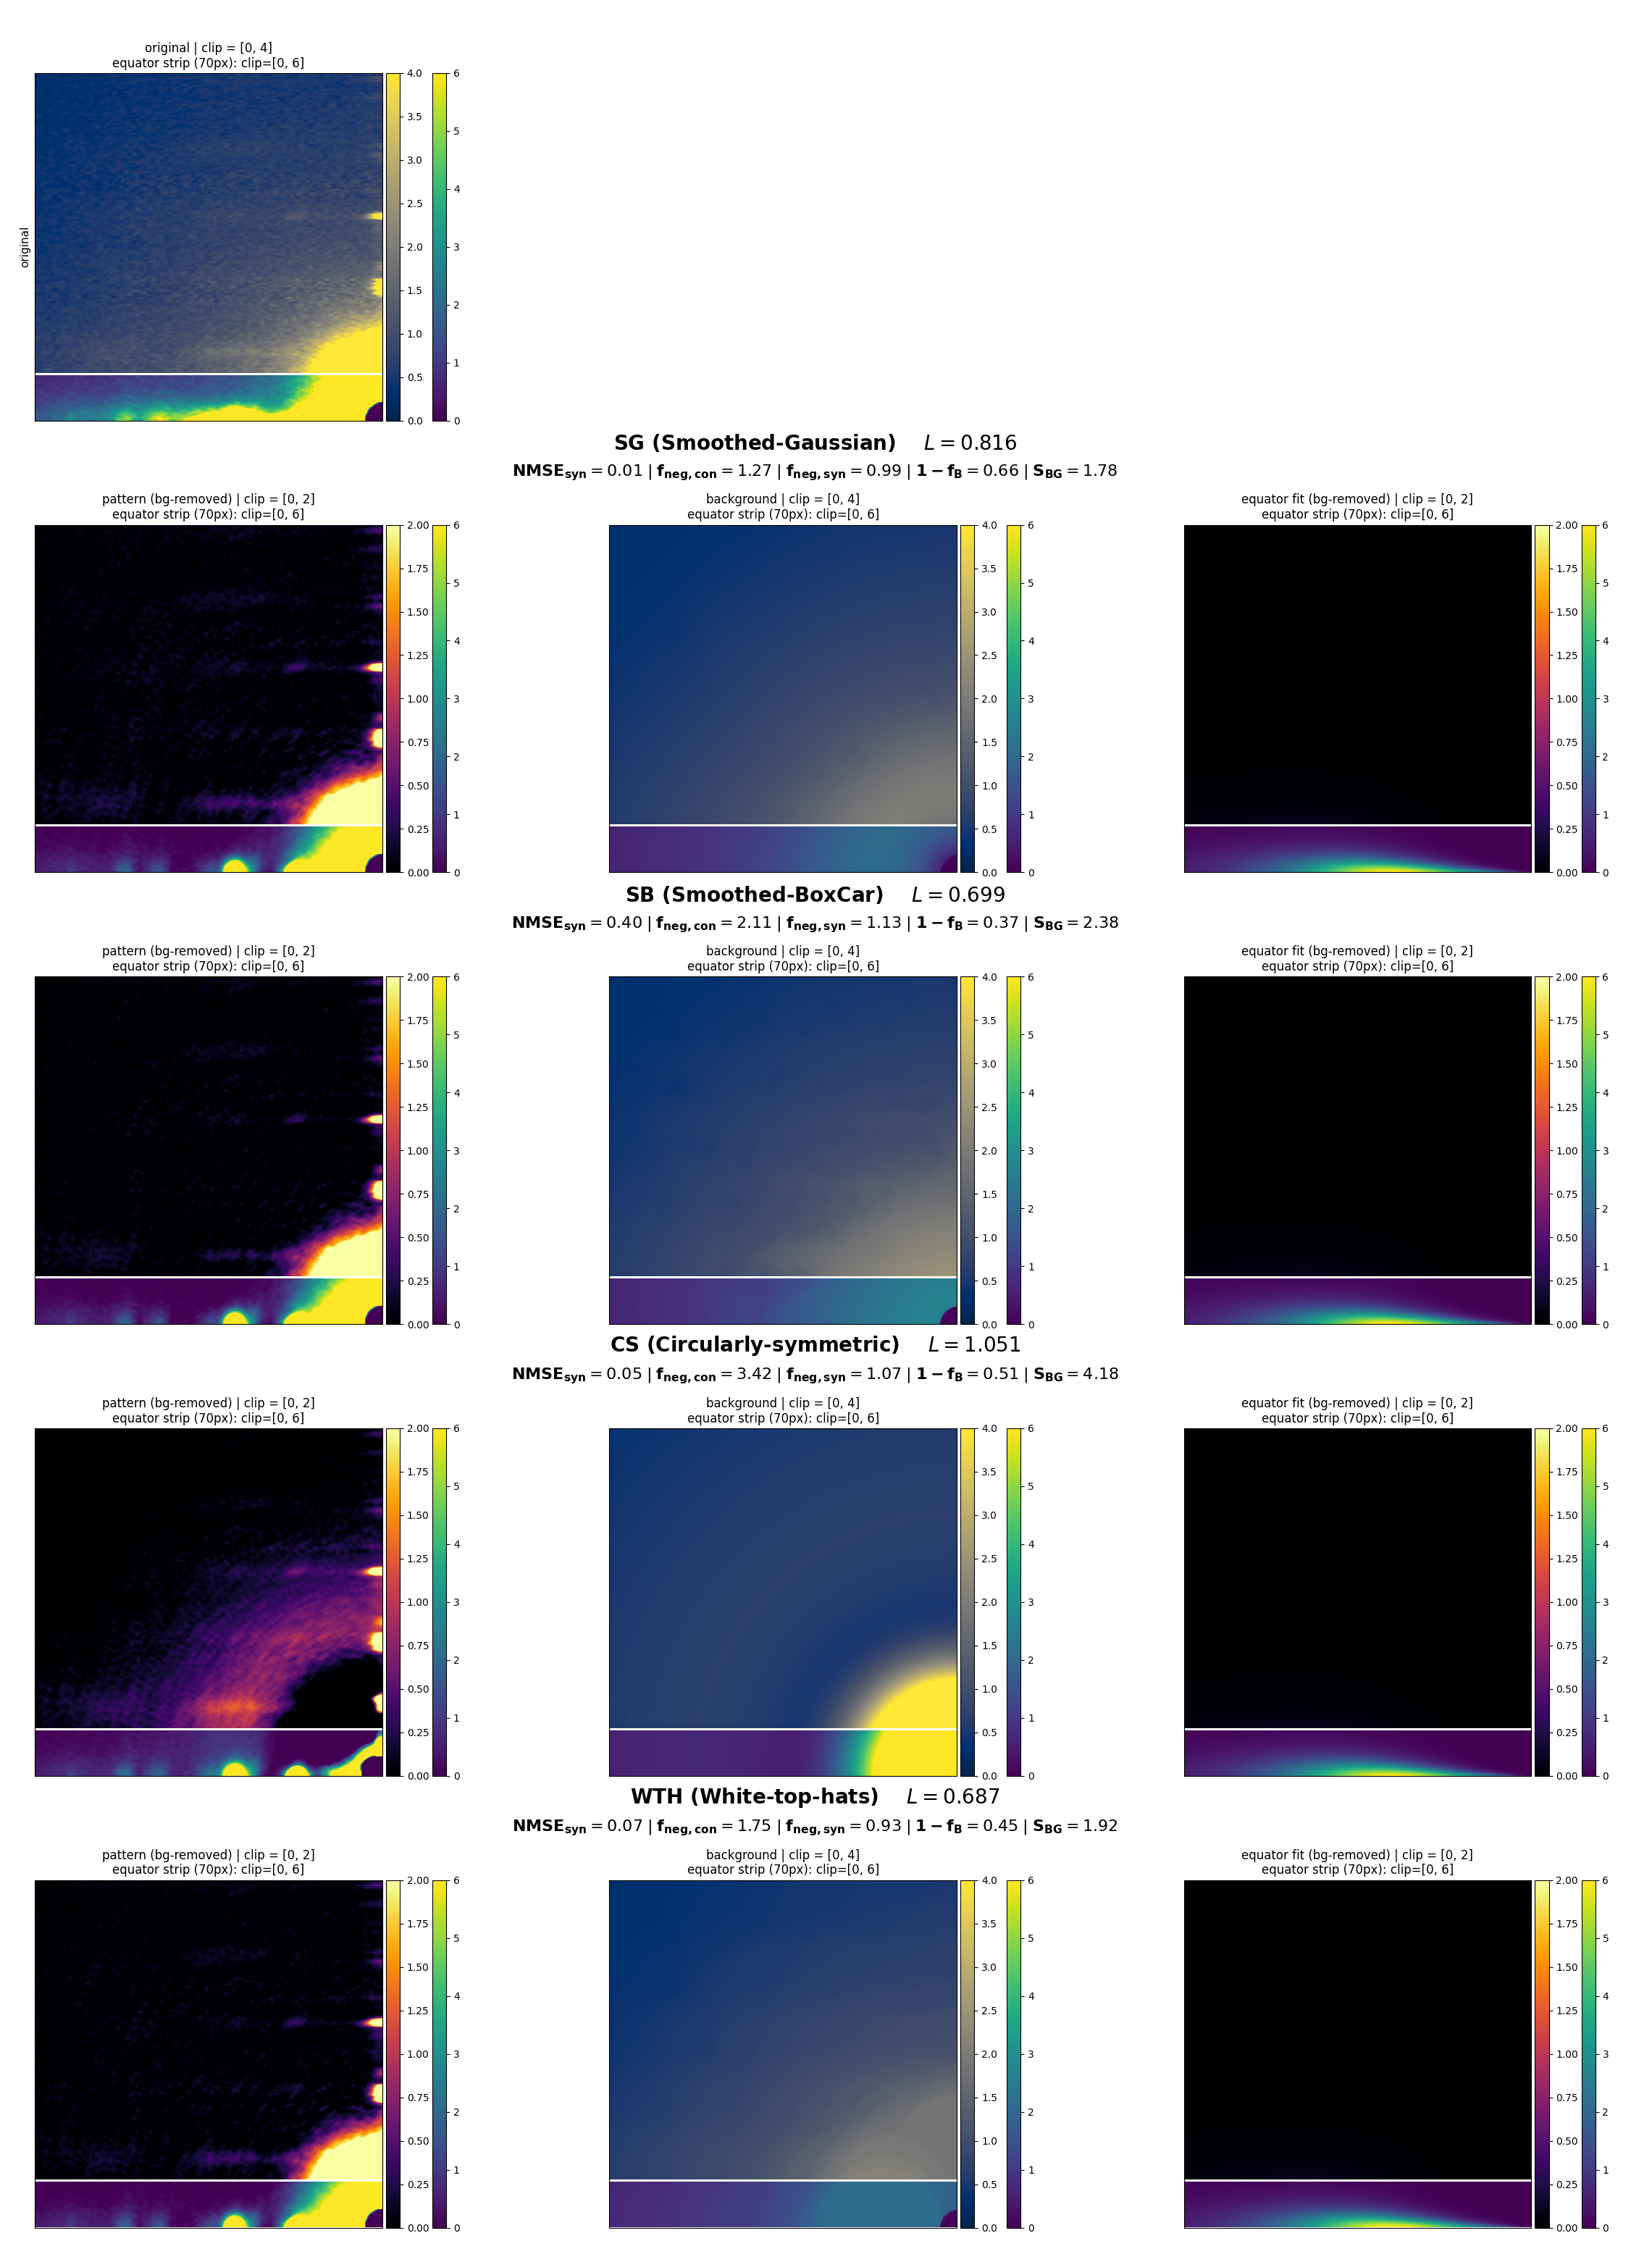
\includegraphics[height=0.9\textheight]{figs/example_eq_Granzier_10_1.png}
% \caption{Visual comparison of background subtraction outcomes for image from dataset 2022\_1028 after equatorial streak fitting and general background removal. Left to right: background-subtracted pattern, background, fitted equatorial streak. The original image is shown at the top. Two scales are used for visualization due to high intensity differences between the background, the equatorial streak and the rest of the pattern.}
% \label{fig:visual_eq_2}
% \end{figure}

% \begin{figure}[htbp]
% \centering

% 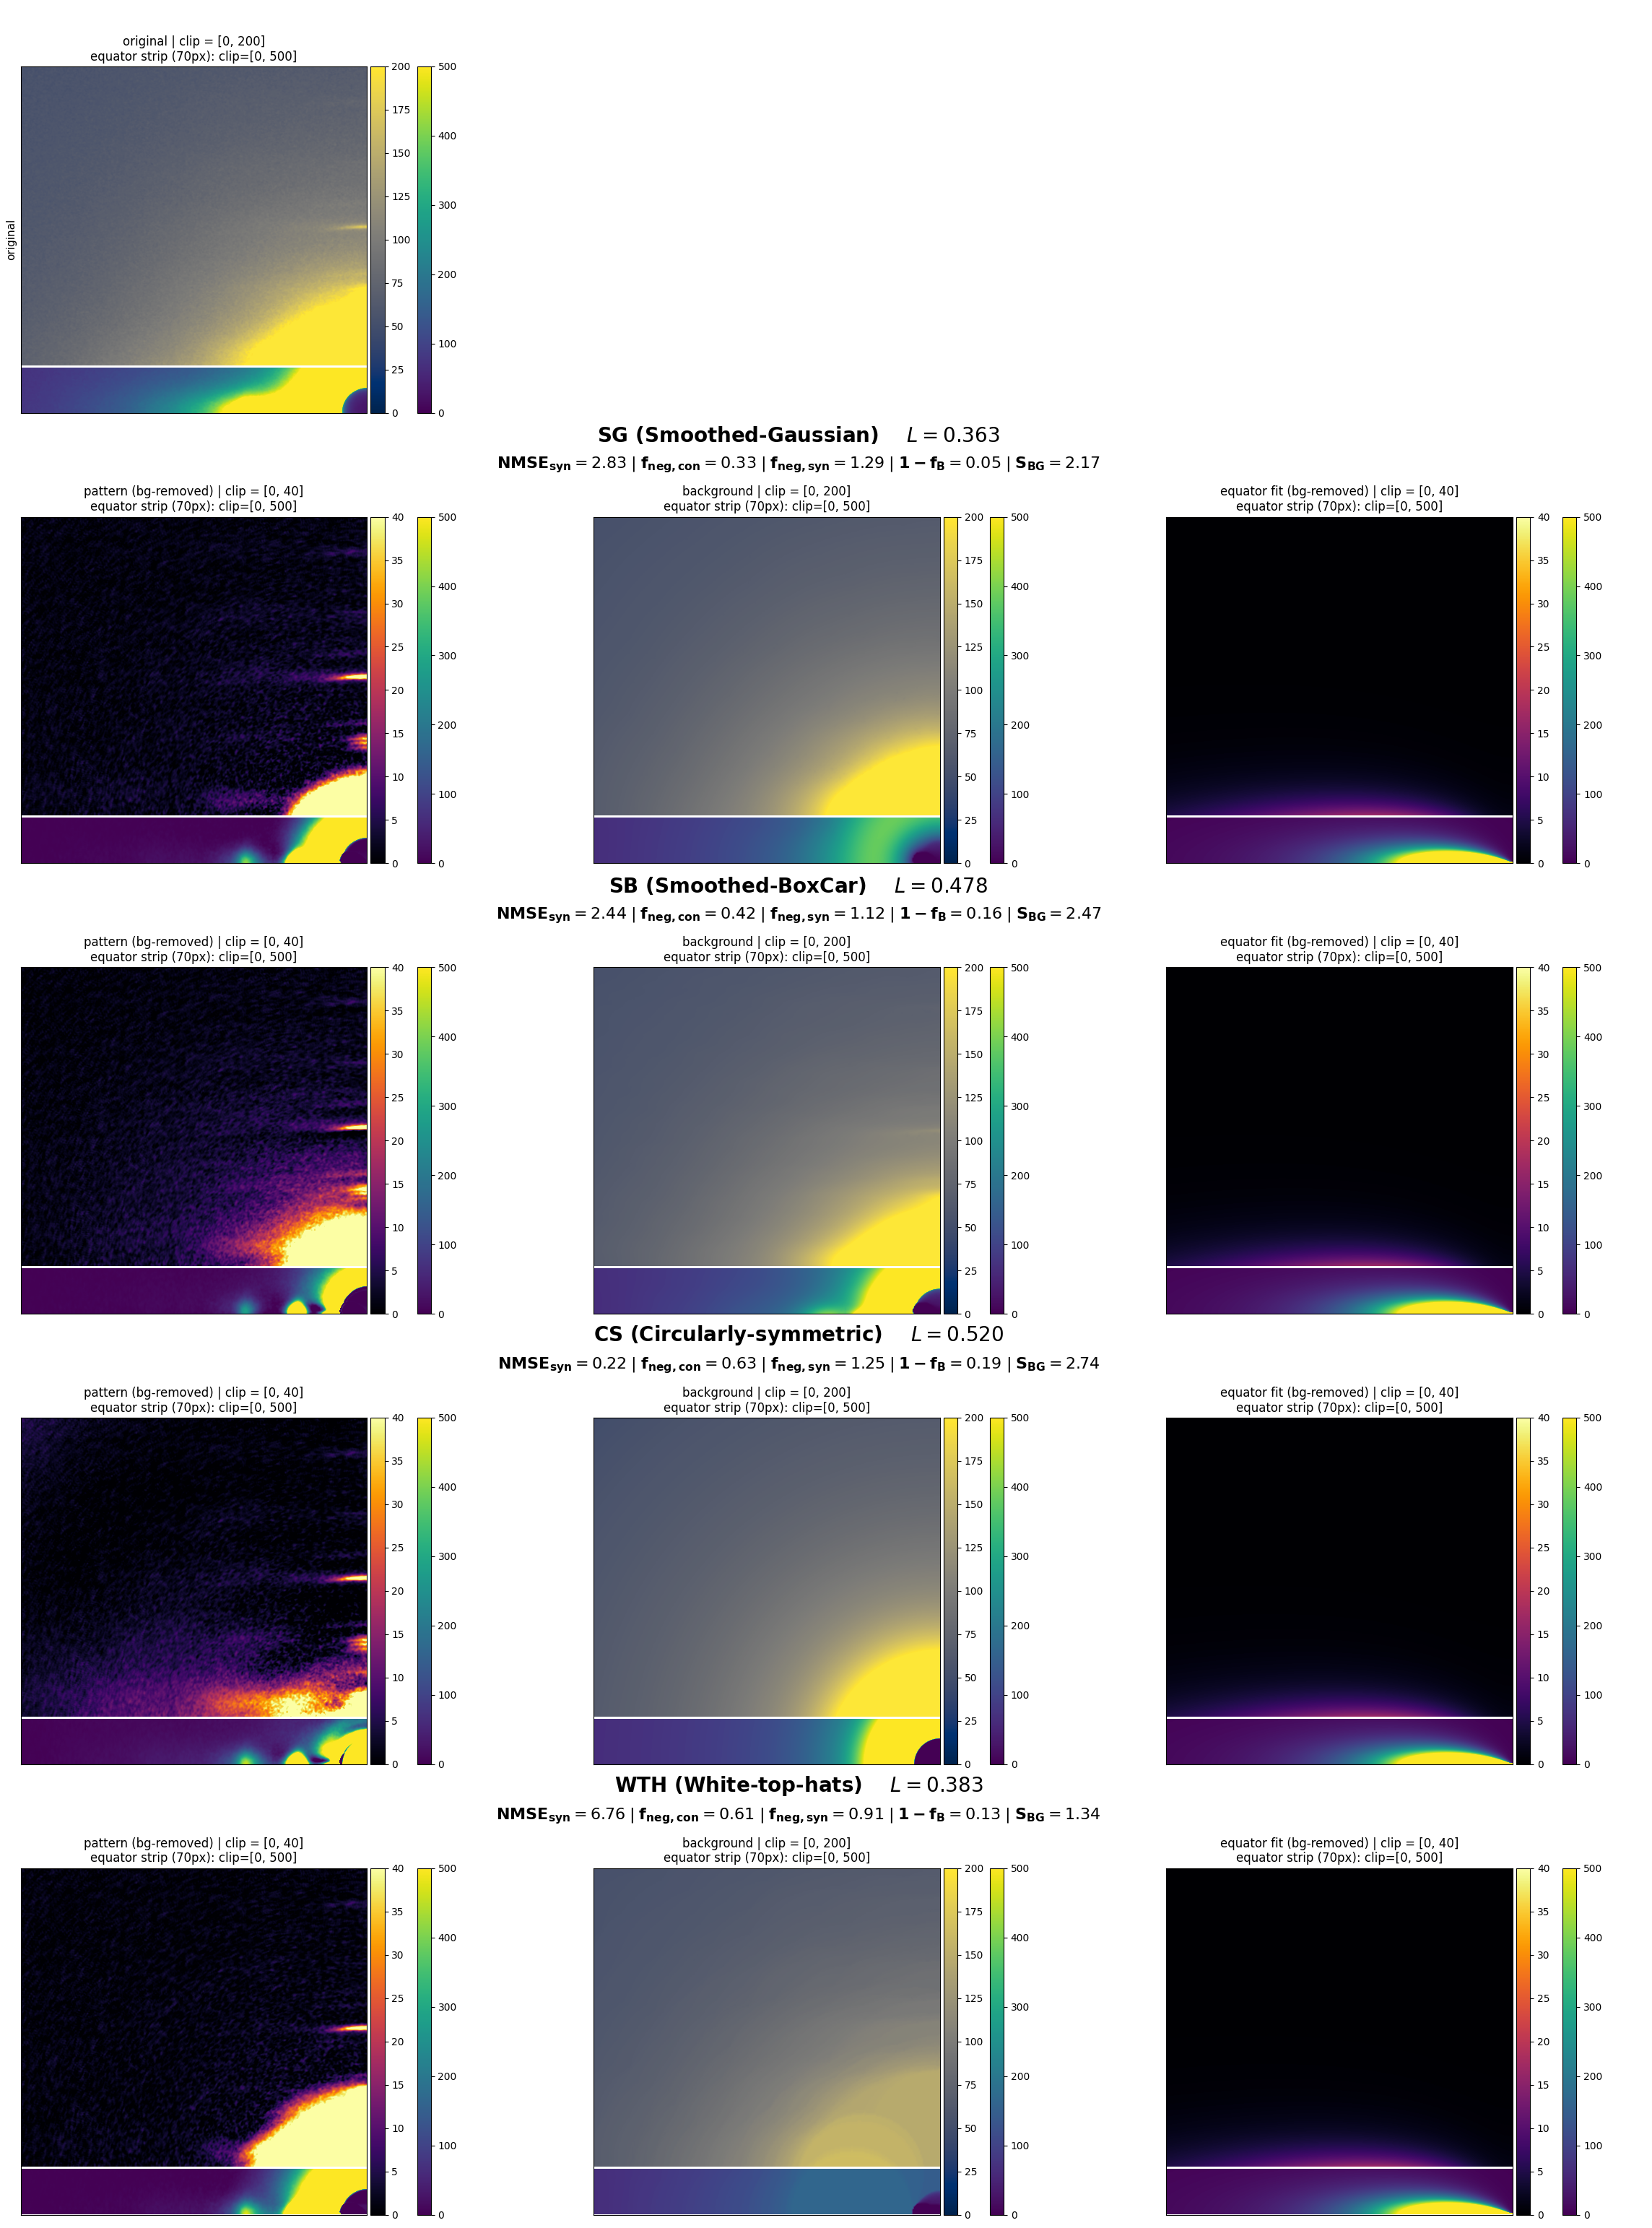
\includegraphics[height=0.9\textheight]{figs/example_eq_MPLL_1_1.png}
% \caption{Visual comparison of background subtraction outcomes for images from dataset MPLL after equatorial streak fitting and general background removal. Left to right: background-subtracted pattern, background, fitted equatorial streak. The original image is shown at the top. Two scales are used for visualization due to high intensity differences between the background, the equatorial streak and the rest of the pattern.}
% \label{fig:visual_eq_3}
% \end{figure}



\begin{figure}[htbp]
\centering
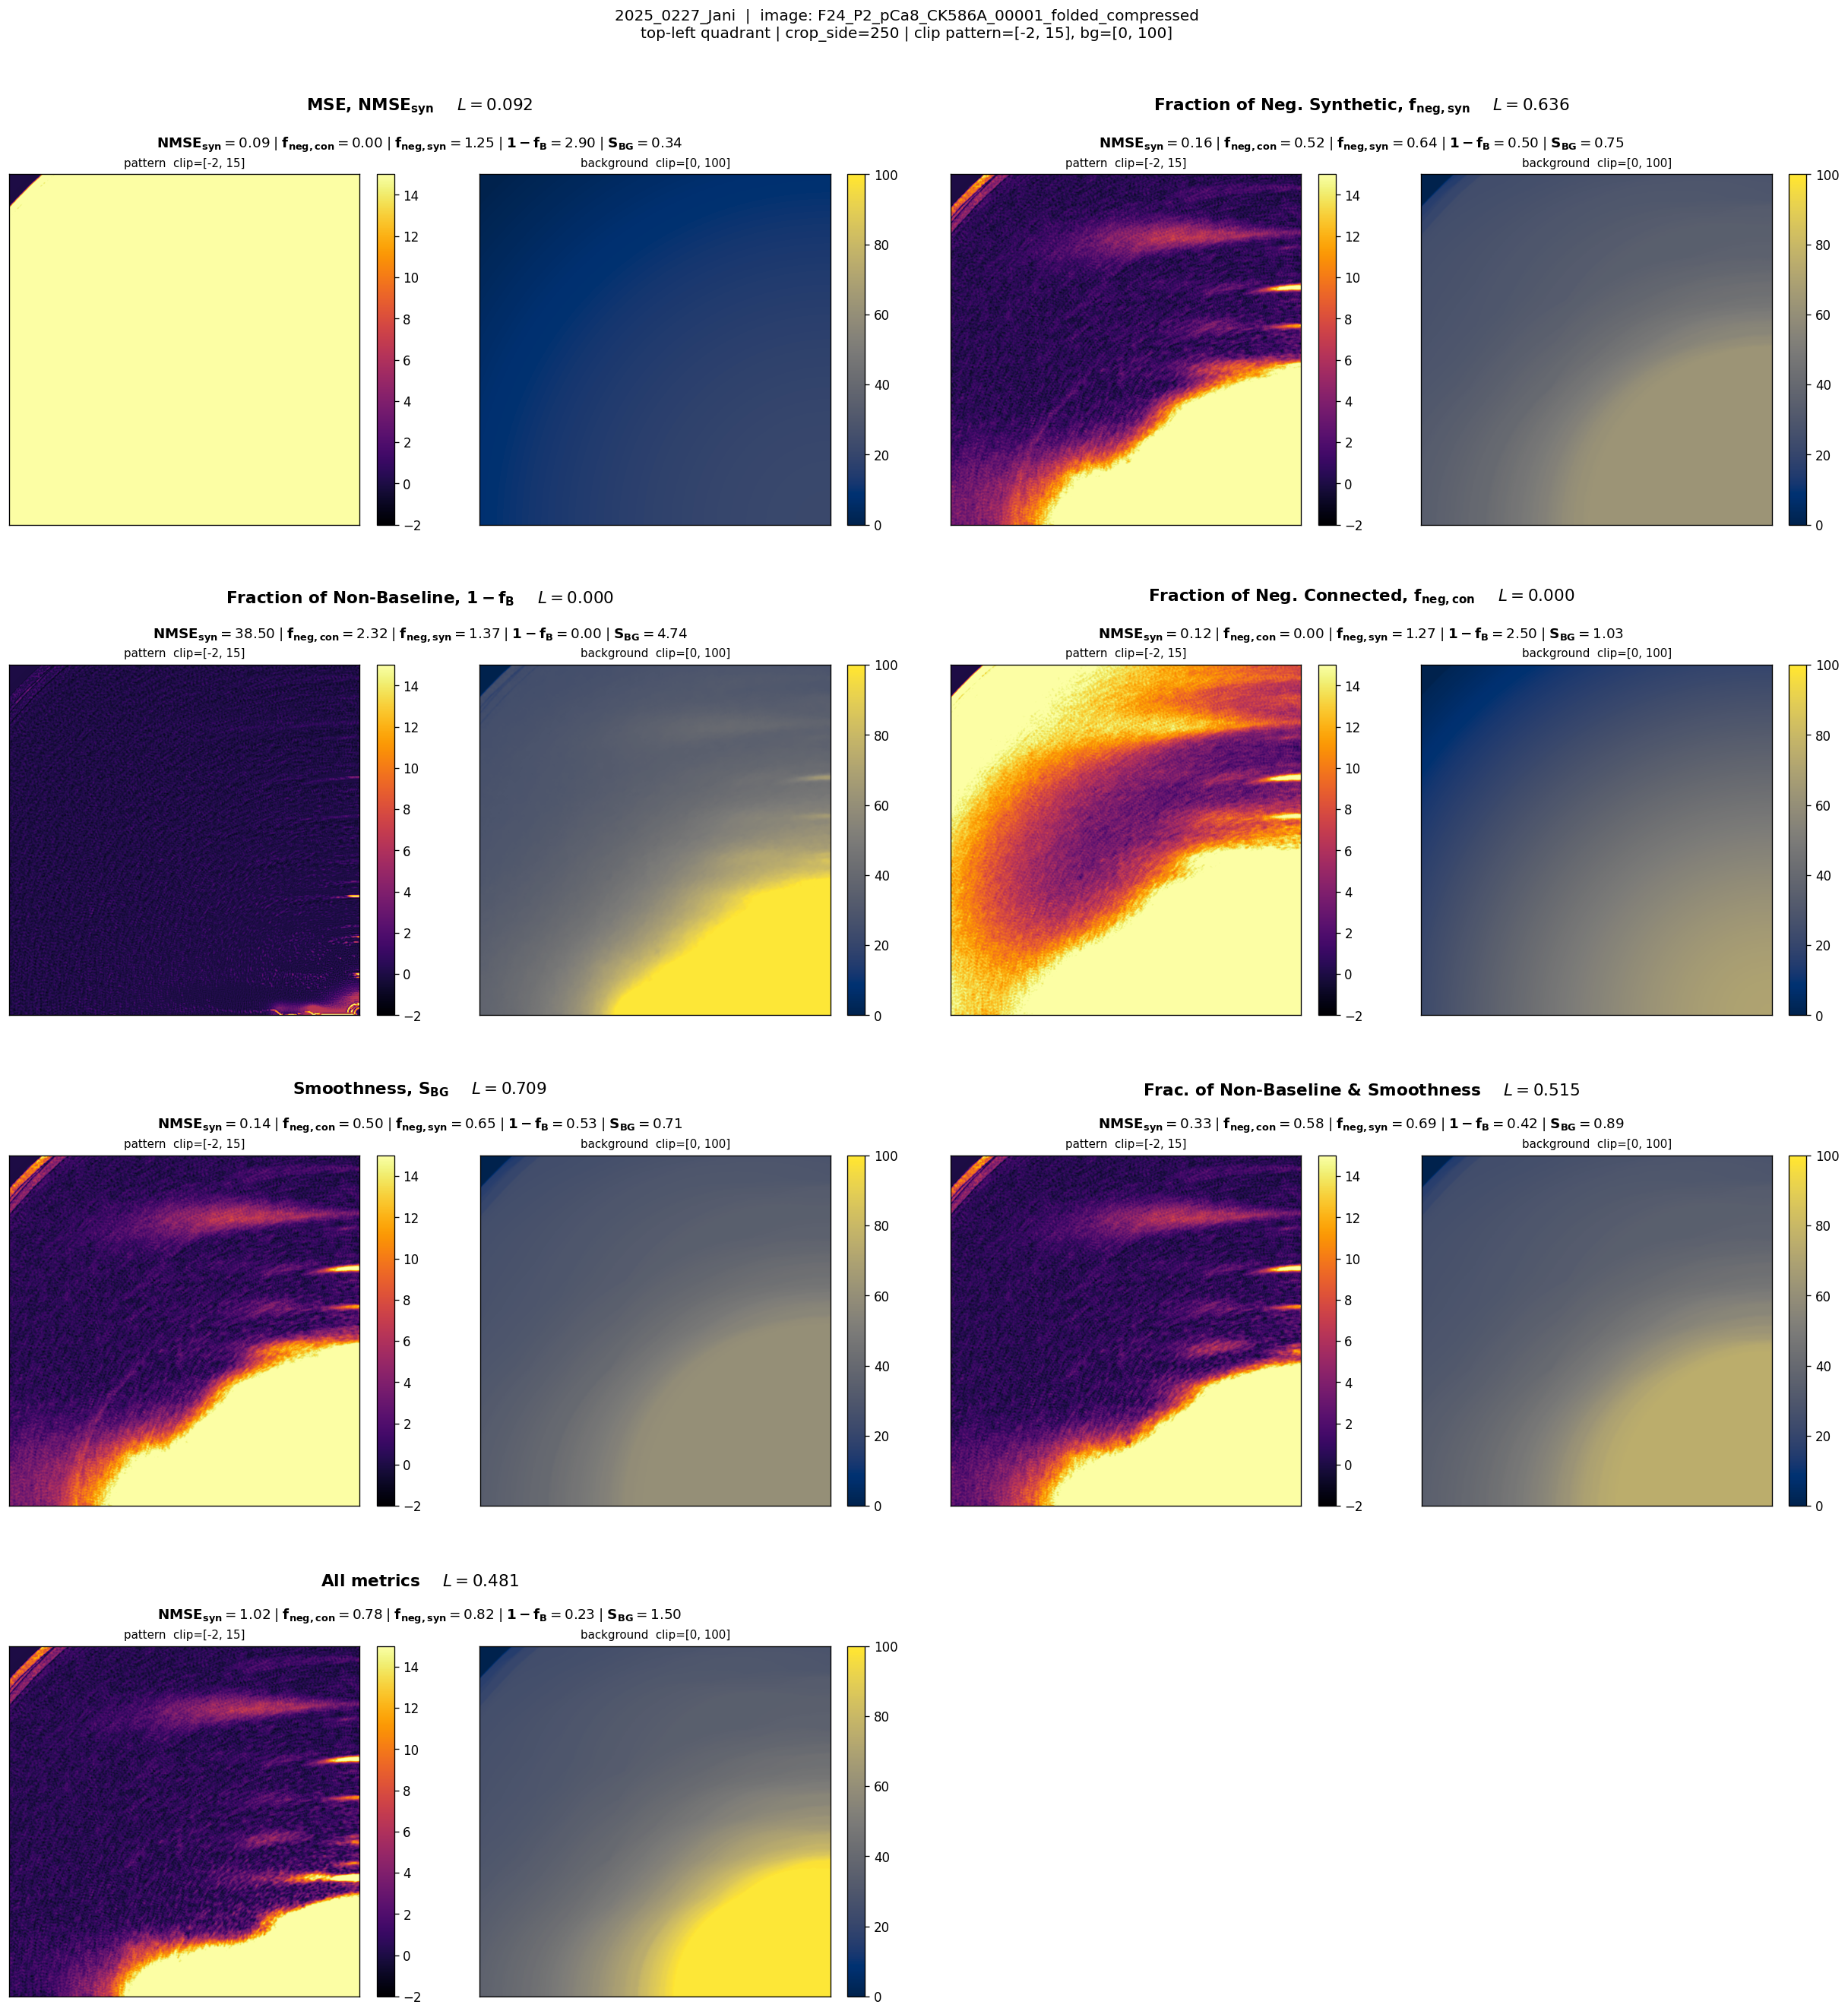
\includegraphics[width=0.9\textwidth]{figs/individual_metrics.png}
\caption{Image sample from dataset 2025\_0227 when guided using metrics individually or a combination of the two most significant. Left of each pair: Background removed image. Right: Background.}
\label{fig:example_1img_metrics}
\end{figure}



\begin{figure}[htbp]
\centering

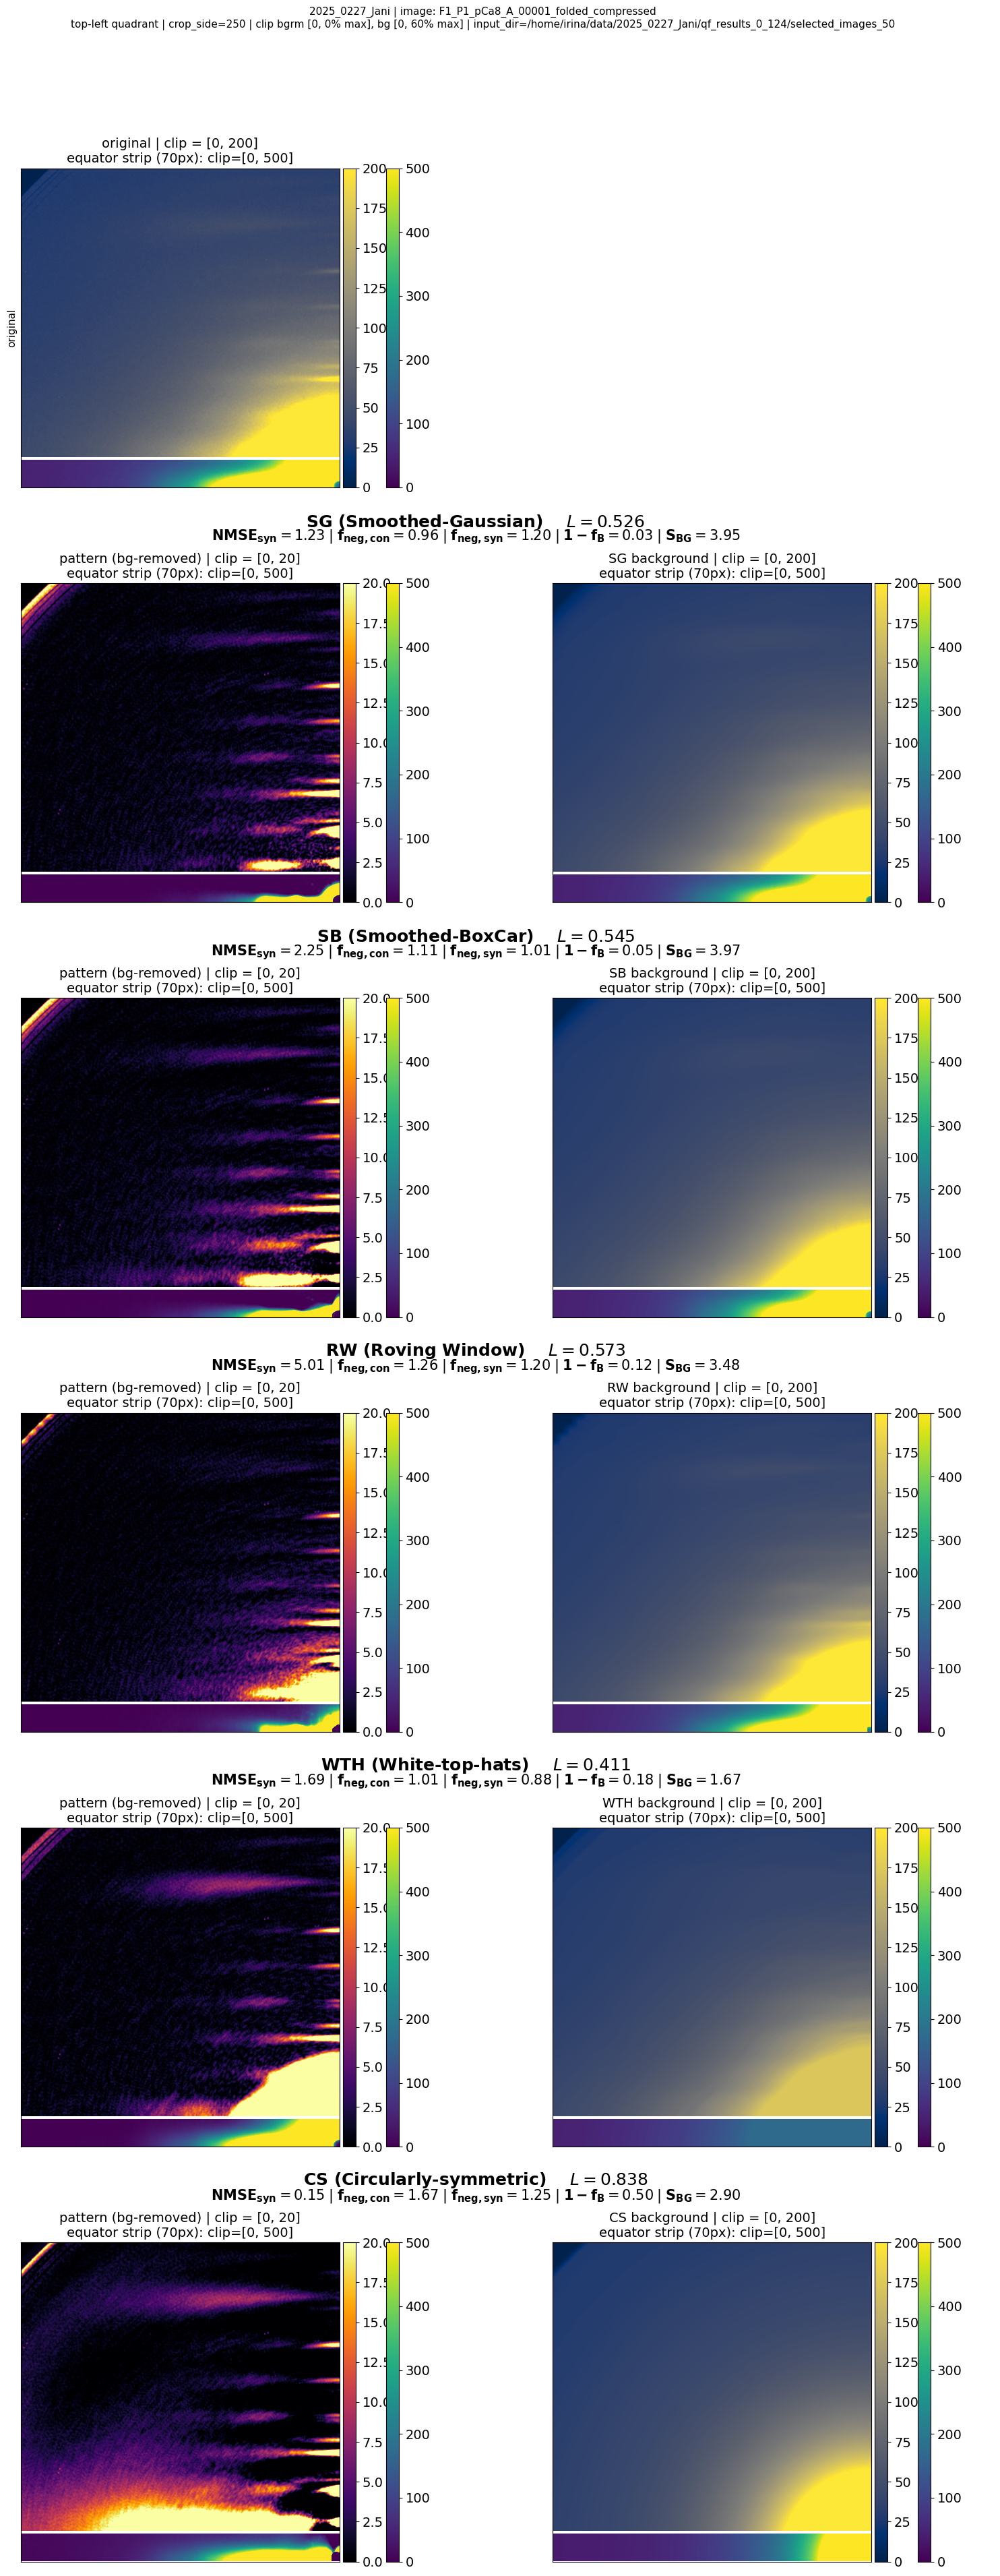
\includegraphics[height=0.9\textheight]{figs/example_no_eq_Jani_0_1_v2.png}
\caption{Visual comparison of background subtraction outcomes for image from dataset 2025\_0402. Left to right: background-sutracted pattern, background. The original image is shown at the top. Two scales are used for visualization due to high intensity differences between the background, the equatorial streak and the rest of the pattern.}
\label{fig:visual_no_eq_1}
\end{figure}


% \begin{figure}[htbp]
% \centering
% 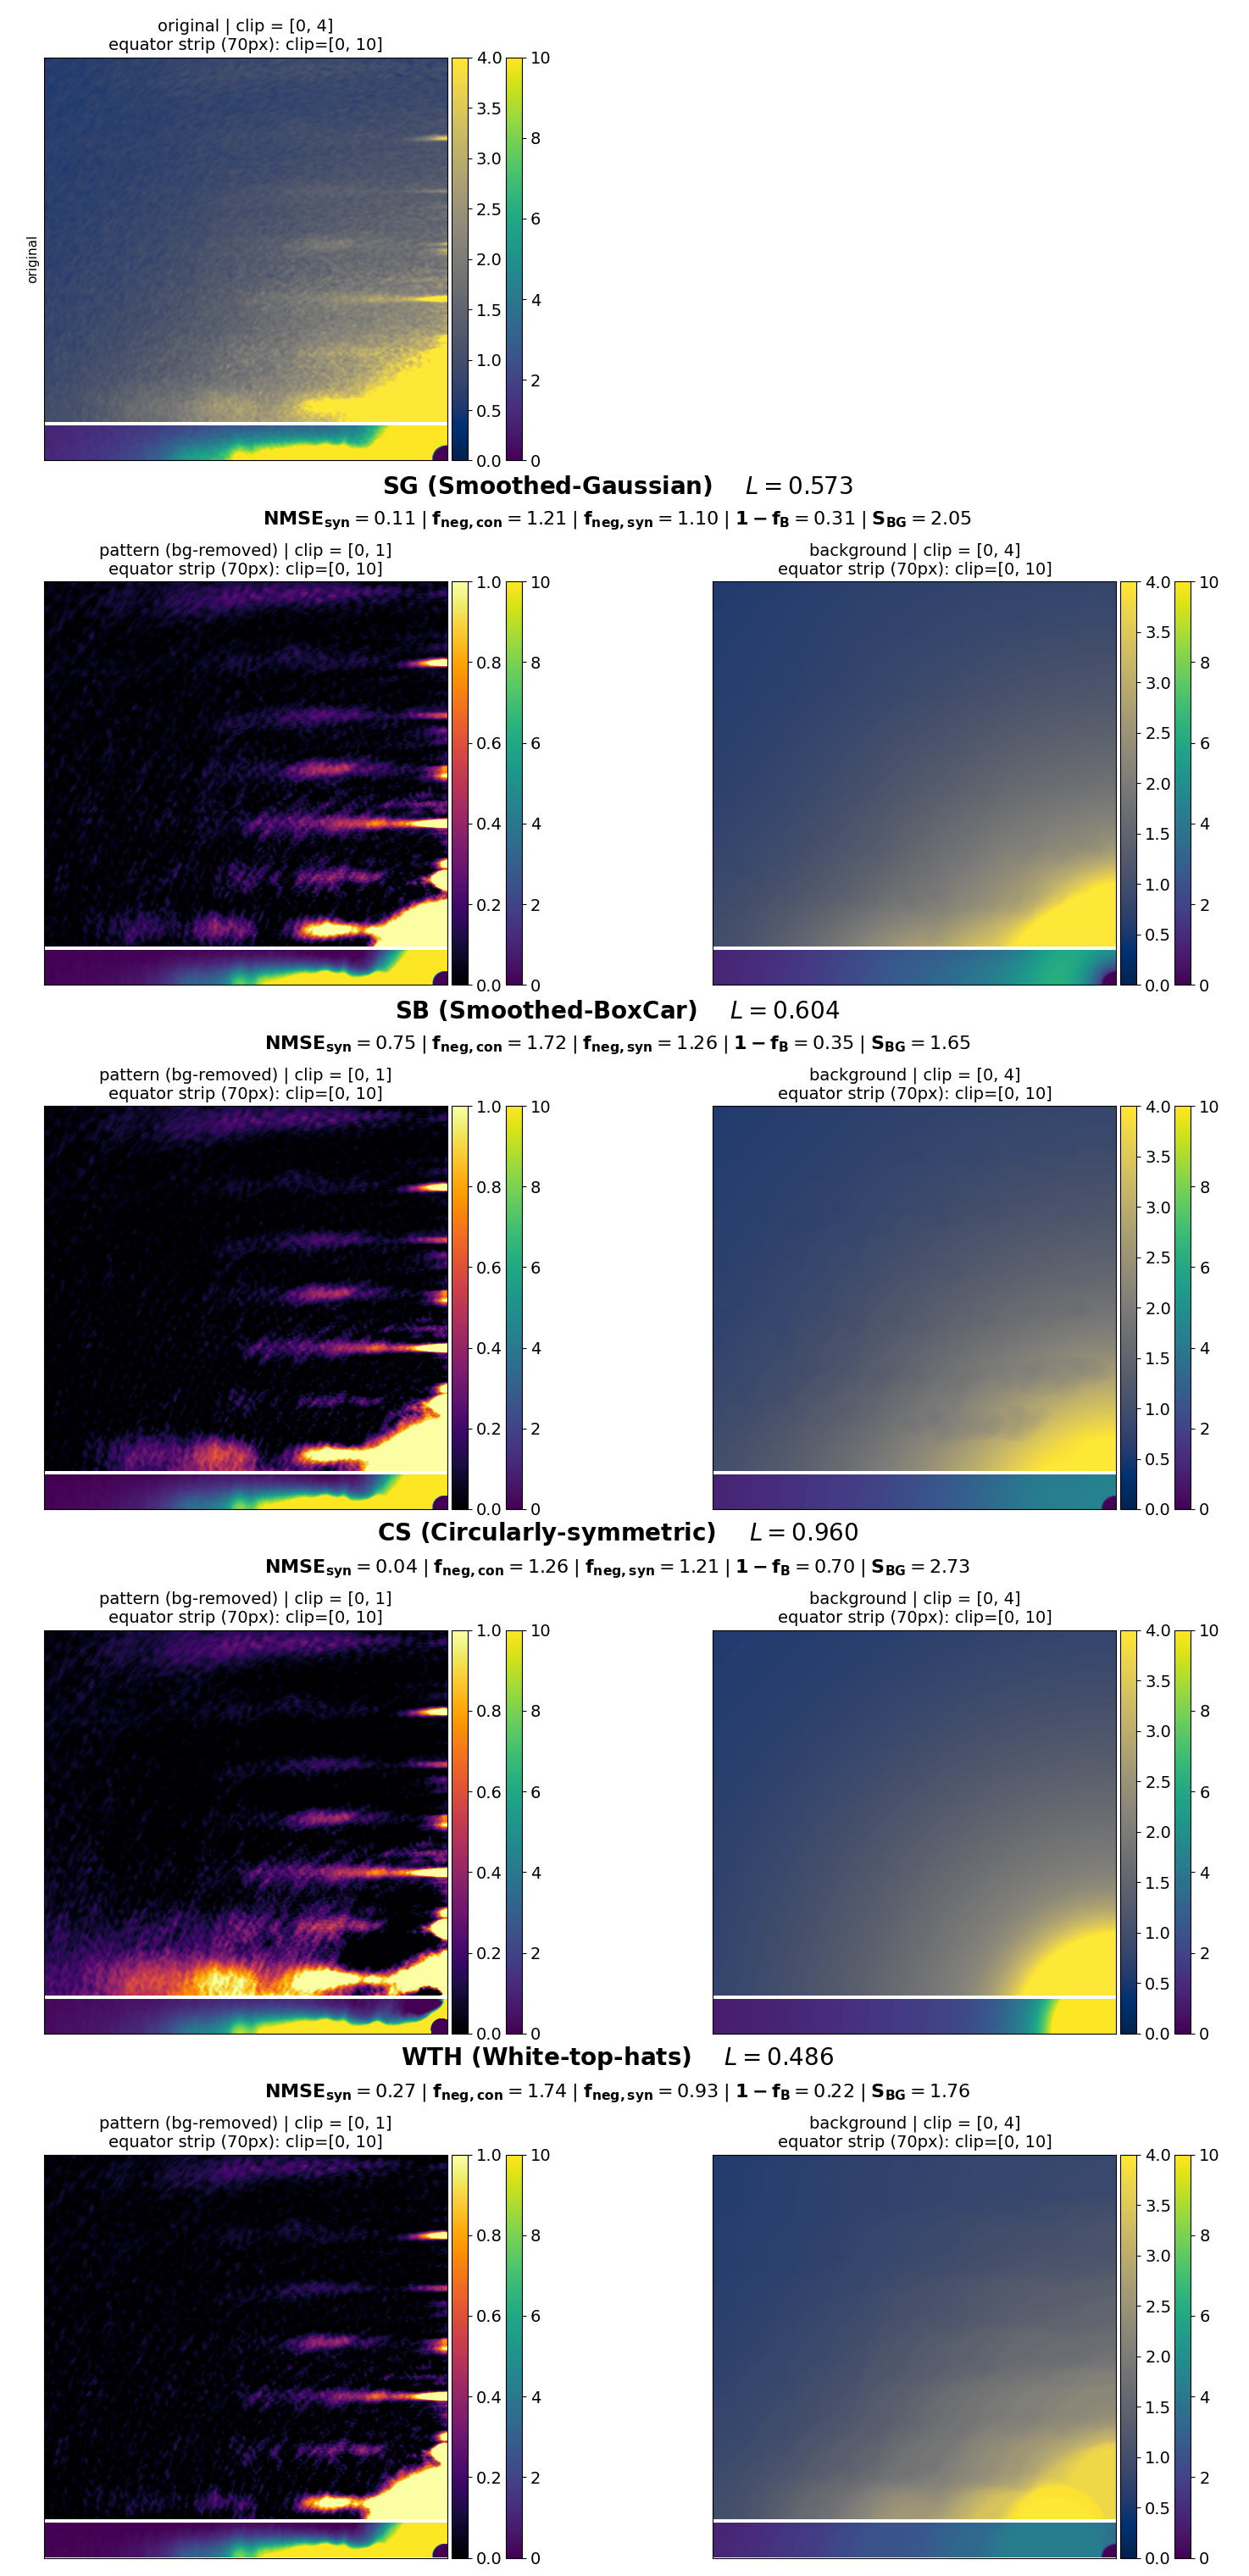
\includegraphics[height=0.9\textheight]{figs/example_no_eq_Granzier_21_1.png}
% \caption{Visual comparison of background subtraction outcomes for image from dataset 2022\_1028. Left to right: background-sutracted pattern, background. The original image is shown at the top. Two scales are used for visualization due to high intensity differences between the background, the equatorial streak and the rest of the pattern.}
% \label{fig:visual_no_eq_2}
% \end{figure}

% \begin{figure}[htbp]
% \centering

% 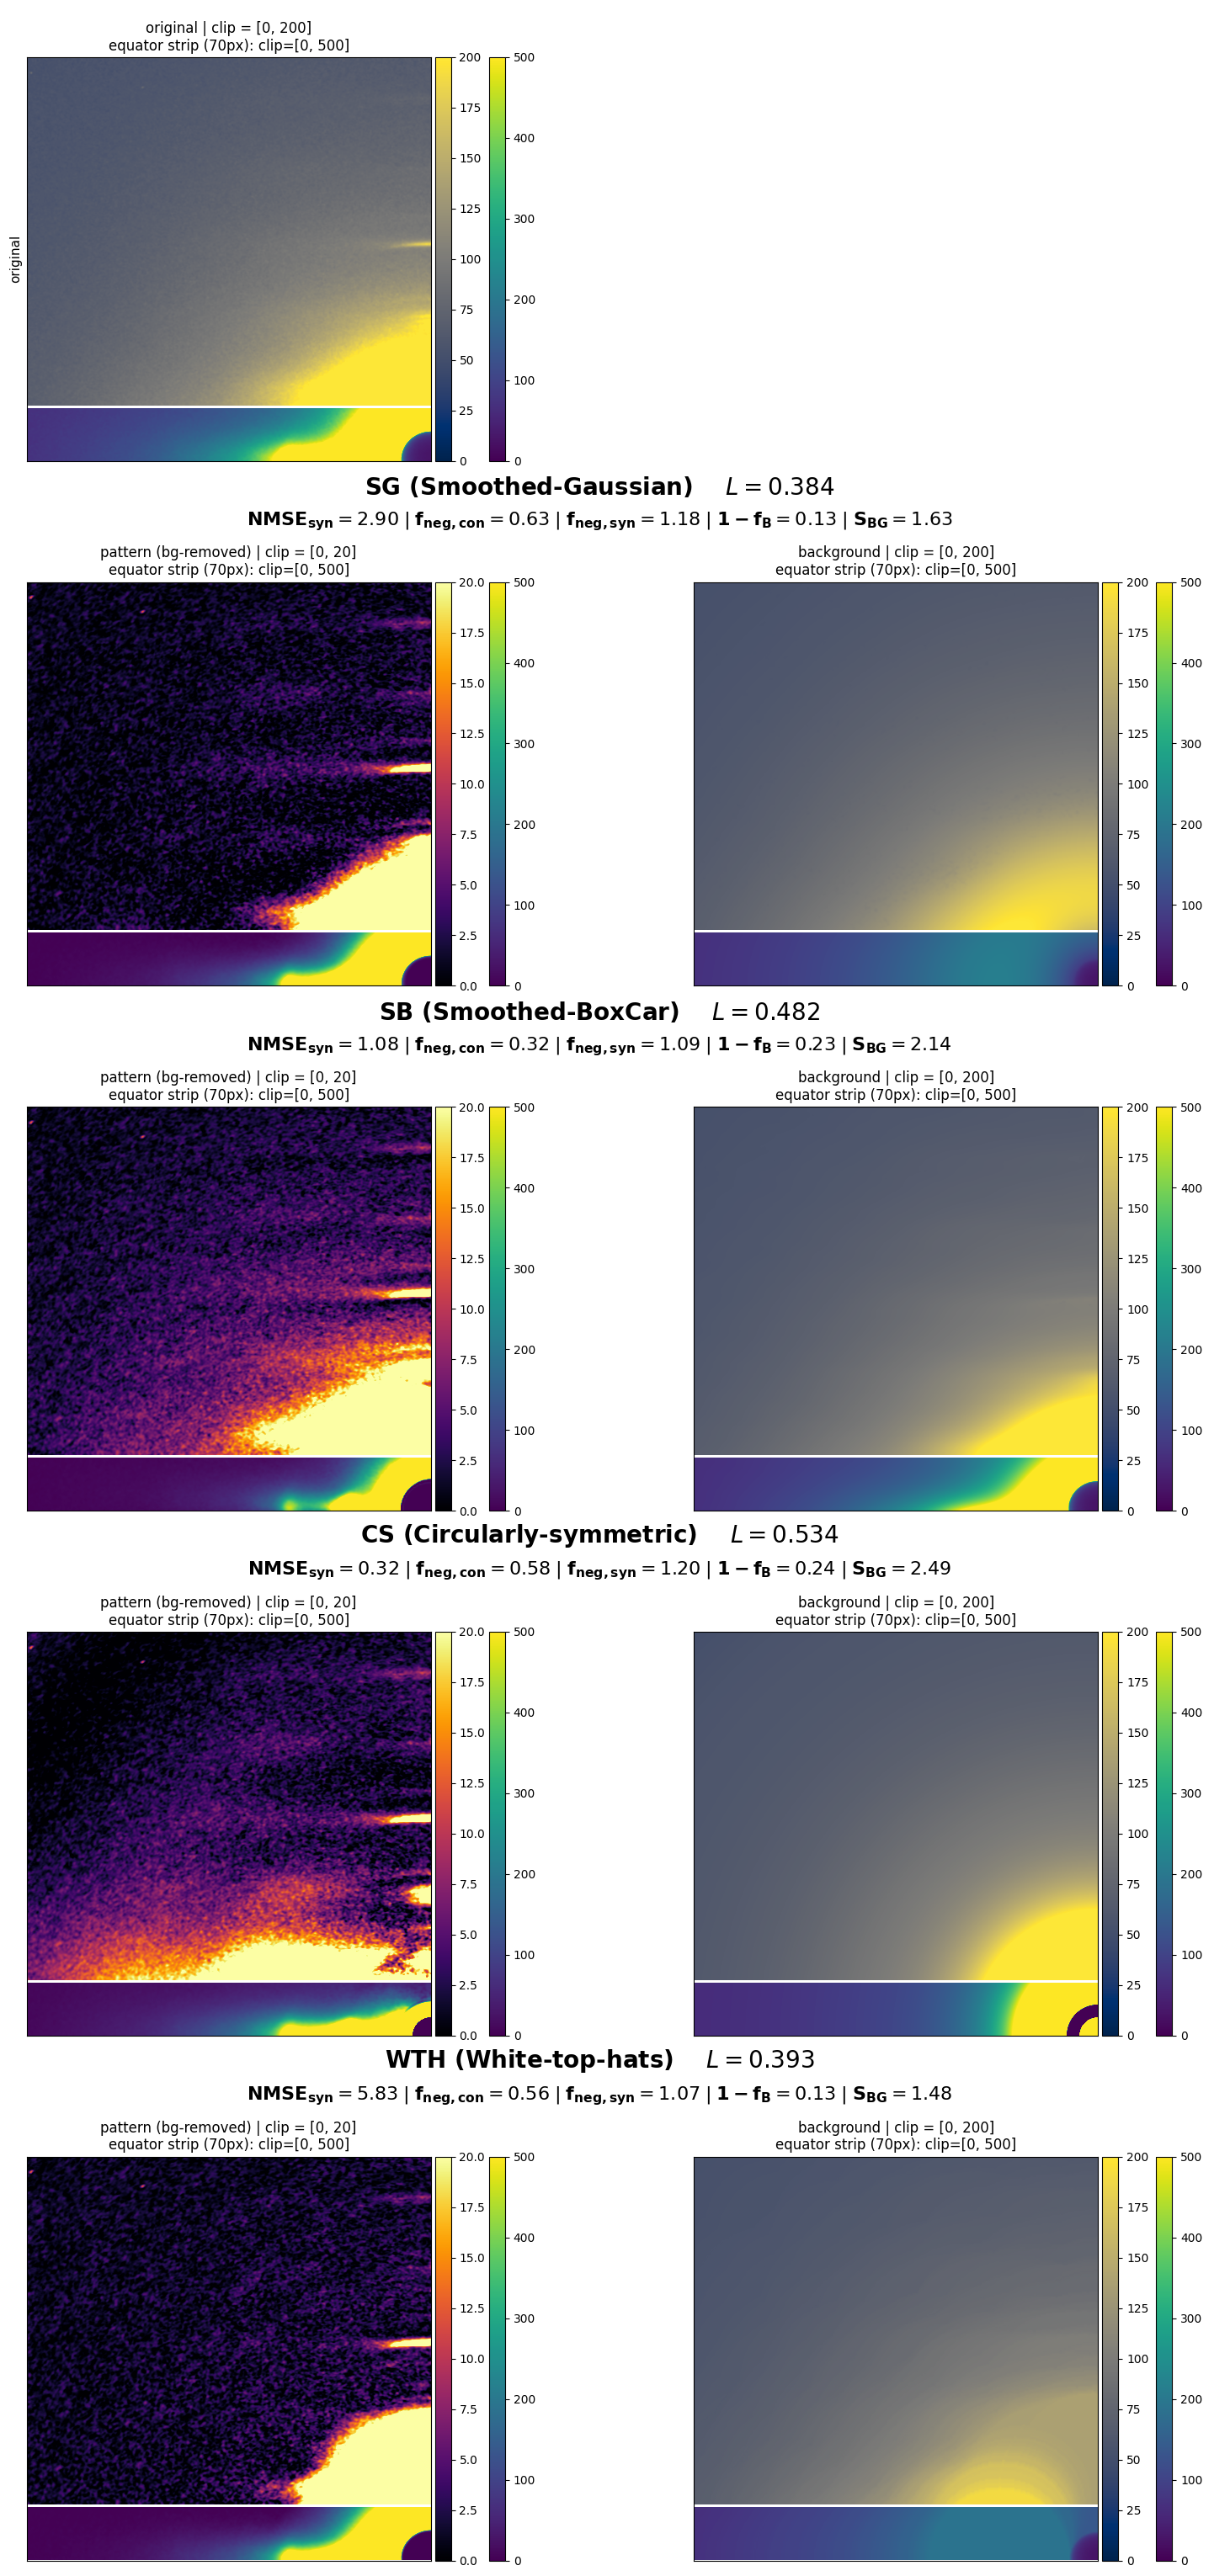
\includegraphics[height=0.9\textheight]{figs/example_no_eq_MPLL_3_1.png}
% \caption{Visual comparison of background subtraction outcomes for images from dataset MPLL. Left to right: background-sutracted pattern, background. The original image is shown at the top. Two scales are used for visualization due to high intensity differences between the background, the equatorial streak and the rest of the pattern.}
% \label{fig:visual_no_eq_3}
% \end{figure}
